\chapter{Změna směru pole při jeho konstantní velikosti} \label{kap_toceni}

V této kapitole vyzkoušíme nový typ magnetooptického měření, který plně využívá výhody dvoudimenzionality elektromagnetu. Elektromagnet umožňuje při konstantní velikosti pole $\mu_0 \hext=\SI{50}{\milli\tesla}$, nebo \SI{210}{\milli\tesla} plynule měnit směr pole od $\phH=\ang{270}$ po směru hodinových ručiček do \ang{-90}, tedy plný rozsah úhlů. V~případě prokázání užitečnosti této metody je možné principiálně zkalibrovat a implementovat i jiné velikosti $\hext$, rozsahy úhlů a smysl otáčení pole (proti směru hodinových ručiček).

Provedli jsme tři měření tohoto druhu
\begin{itemize}
	\item $\mu_0 \hext=\SI{210}{\milli\tesla}$, $T<\SI{15}{\kelvin}$
	\item $\mu_0 \hext=\SI{50}{\milli\tesla}$, $T<\SI{15}{\kelvin}$
	\item $\mu_0 \hext=\SI{210}{\milli\tesla}$, $T=\SI{38,7(10)}{\kelvin}$
\end{itemize}
První dvě uvedená měření proběhla ve stejný den při stejném zchlazení vzorku.

Měření proběhlo v kolineární geometrii a intenzita laseru dopadajícího na vzorek byla \SI{1,2}{\milli\watt}.



\section{Teoretický popis}
Pomocí optického můstku změříme při daném průběhu pole klasicky rozdílový a součtový signál. Toto provedeme pro více polarizací $\beta \in (\ang{0}, \ang{180})$ s krokem \ang{15}.

Teď bychom rozdílový a součtový signál rádi převedli na veličiny $\Delta \beta$ a $B$ podobně jako v hysterezních smyčkách, ale narážíme na problém. V našem experimentu potřebujeme správně určit hladinu $\Delta \beta=0$, tzn. vyvážit můstek tak, aby nulové rozdílové napětí odpovídalo situaci, kdy dopadající a odražené světlo je lineárně polarizované ve stejné rovině. S veličinou $B$ narážíme na stejný nedostatek. 

Nabízí se možnost jako nulovou hladinu zvolit střední hodnotu každé křivky. Střední hodnotu ale počítáme vzhledem k $\phH$ a ne $\phM$, a proto nemusí být nutně nulová.
V každém bodě změřené křivky má magnetizace určitý definovaný směr a tedy existuje zatím neznámá funkční závislost $\phM(\phH)$. Podle \eqref{rotace_polarizace} platí
\begin{equation}
\Delta \beta(\phH, \beta) = \pmld \sin \left[ 2(\phM(\phH)-\beta) \right] \,.
\end{equation}
Střední hodnota naměřené křivky vzhledem k $\phH$ je tedy
\begin{equation}
\begin{aligned}
\str{\Delta\beta} &= \str{\pmld \sin \left[ 2(\phM-\beta) \right]} \\
&= \str{\pmld \sin(2\phM)\cos(2\beta)-\cos(2\phM)\sin(2\beta)} \\
&=  \str{\pmld\sin(2\phM)}\cos(2\beta)- \str{\pmld\cos(2\phM)}\sin(2\beta) \\
&=K \sin\left[ 2(\alpha-\beta) \right] \,, \\
\end{aligned}
\end{equation}
kde uvažujeme, že $\pmld$ může záviset na směru magnetizace a tím pádem i směru vnějšího pole. Označili jsme
\begin{equation}
\begin{aligned}
K&=\sqrt{ \str{\pmld\sin(2\phM) }^2 +  \str{\pmld\cos(2\phM) }^2 } \\
\tan(2\alpha) &=\frac{\str{\pmld\sin(2\phM) }}{\str{\pmld\cos(2\phM) }}
\end{aligned}
\end{equation}

Pokud zvolíme jako nulovou hladinu $\Delta\beta$ její střední hodnotu, dostaneme veličinu, pro kterou platí
\begin{equation}
\left[ \Delta \beta - \str{\Delta\beta}  \right](\phH, \beta)=\pmld \sin[2(\phM-\beta)] - K \sin\left[ 2(\alpha-\beta) \right] \,.
\end{equation}
$\phM(\phH)$ a $\pmld(\phM)$ jsou zatím neurčené hledané závislosti. $K$ a $\alpha$ jsou vzhledem k $\phH$ a $\beta$ konstanty, ale závisí na hledaných $\phM(\phH)$ a $\pmld(\phM)$ v celém rozsahu $\phH$.

Pokud změříme $m$ různých $\phH$ a $n$ různých $\beta$, budeme mít $mn$ hodnot a $2m$ neznámých parametrů $\phM$ a $\pmld$, které by principiálně bylo možné nafitovat. Jednalo by se ovšem o obrovský nelineární fit a výsledky navíc nemusí být jednoznačné.
Výpočetně snazší možností by byla selfkonzistentní metoda. V této práci zatím používáme zjednodušený model.

Vzorek, se kterým pracujeme, má přibližně kubickou symetrii (viz kapitola \ref{kap_vzorek}), tj. je přibližně symetrický při otočení o \ang{90} v rovině $xy$. Je-li tomu tak, pak vymizí konstanta $K$ a platí
\begin{equation} \label{e:asass}
\left[ \Delta \beta - \str{\Delta\beta}  \right](\phH, \beta)=\pmld \sin[2(\phM-\beta)] \,,
\end{equation}
což nám umožňuje fitovat pouze $\phM$ a $\pmld$ v řezech $\phH=\text{konst}$.

Podobně pro $B$
\begin{equation} \label{e:sss}
\left[ B - \str{B}  \right](\phH, \beta)=2\pmld \cos[2(\phM-\beta)] \,.
\end{equation}


\section{Metoda měření a zpracování dat}

Metoda měření i zpracování dat je ve všech třech měřených případech totožná. Čtenáře důkladně provedeme první sadou měření a u zbylých dvou uvedeme pouze výsledky.

Náš vzorek má téměř kubickou symetrii (viz tabulka \ref{tab_vzorek}) a proto použijeme výše uvedený postup.
Měříme vždy rozsah $\phH$ od \ang{270} do \ang{-90} s krokem \ang{5}.

Způsob zpracování dat z tohoto experimentu je oproti měření hysterezních smyček mnohem citlivější na šum (jednotlivé hodnoty změřených bodů i dlouhodobý drift). Proto každé jednotlivé měření provádíme pětkrát za sebou. Změřené křivky zprůměrujeme, tj. pro každé $\phH$ obdržíme hodnotu (rozdílové a součtové napětí) jako průměr z pěti hodnot, z každé změřené křivky jedna pro dané $\phH$.


Součtový a rozdílový signál přepočteme na $\Delta\beta$ a $B$ a od každé z křivek odečteme její střední hodnotu, jak je popsáno výše.
Príklad takových křivek je na obr. \ref{toc_hrube} (a), (b). 


\begin{figure}[htbp]\centering
\qq{	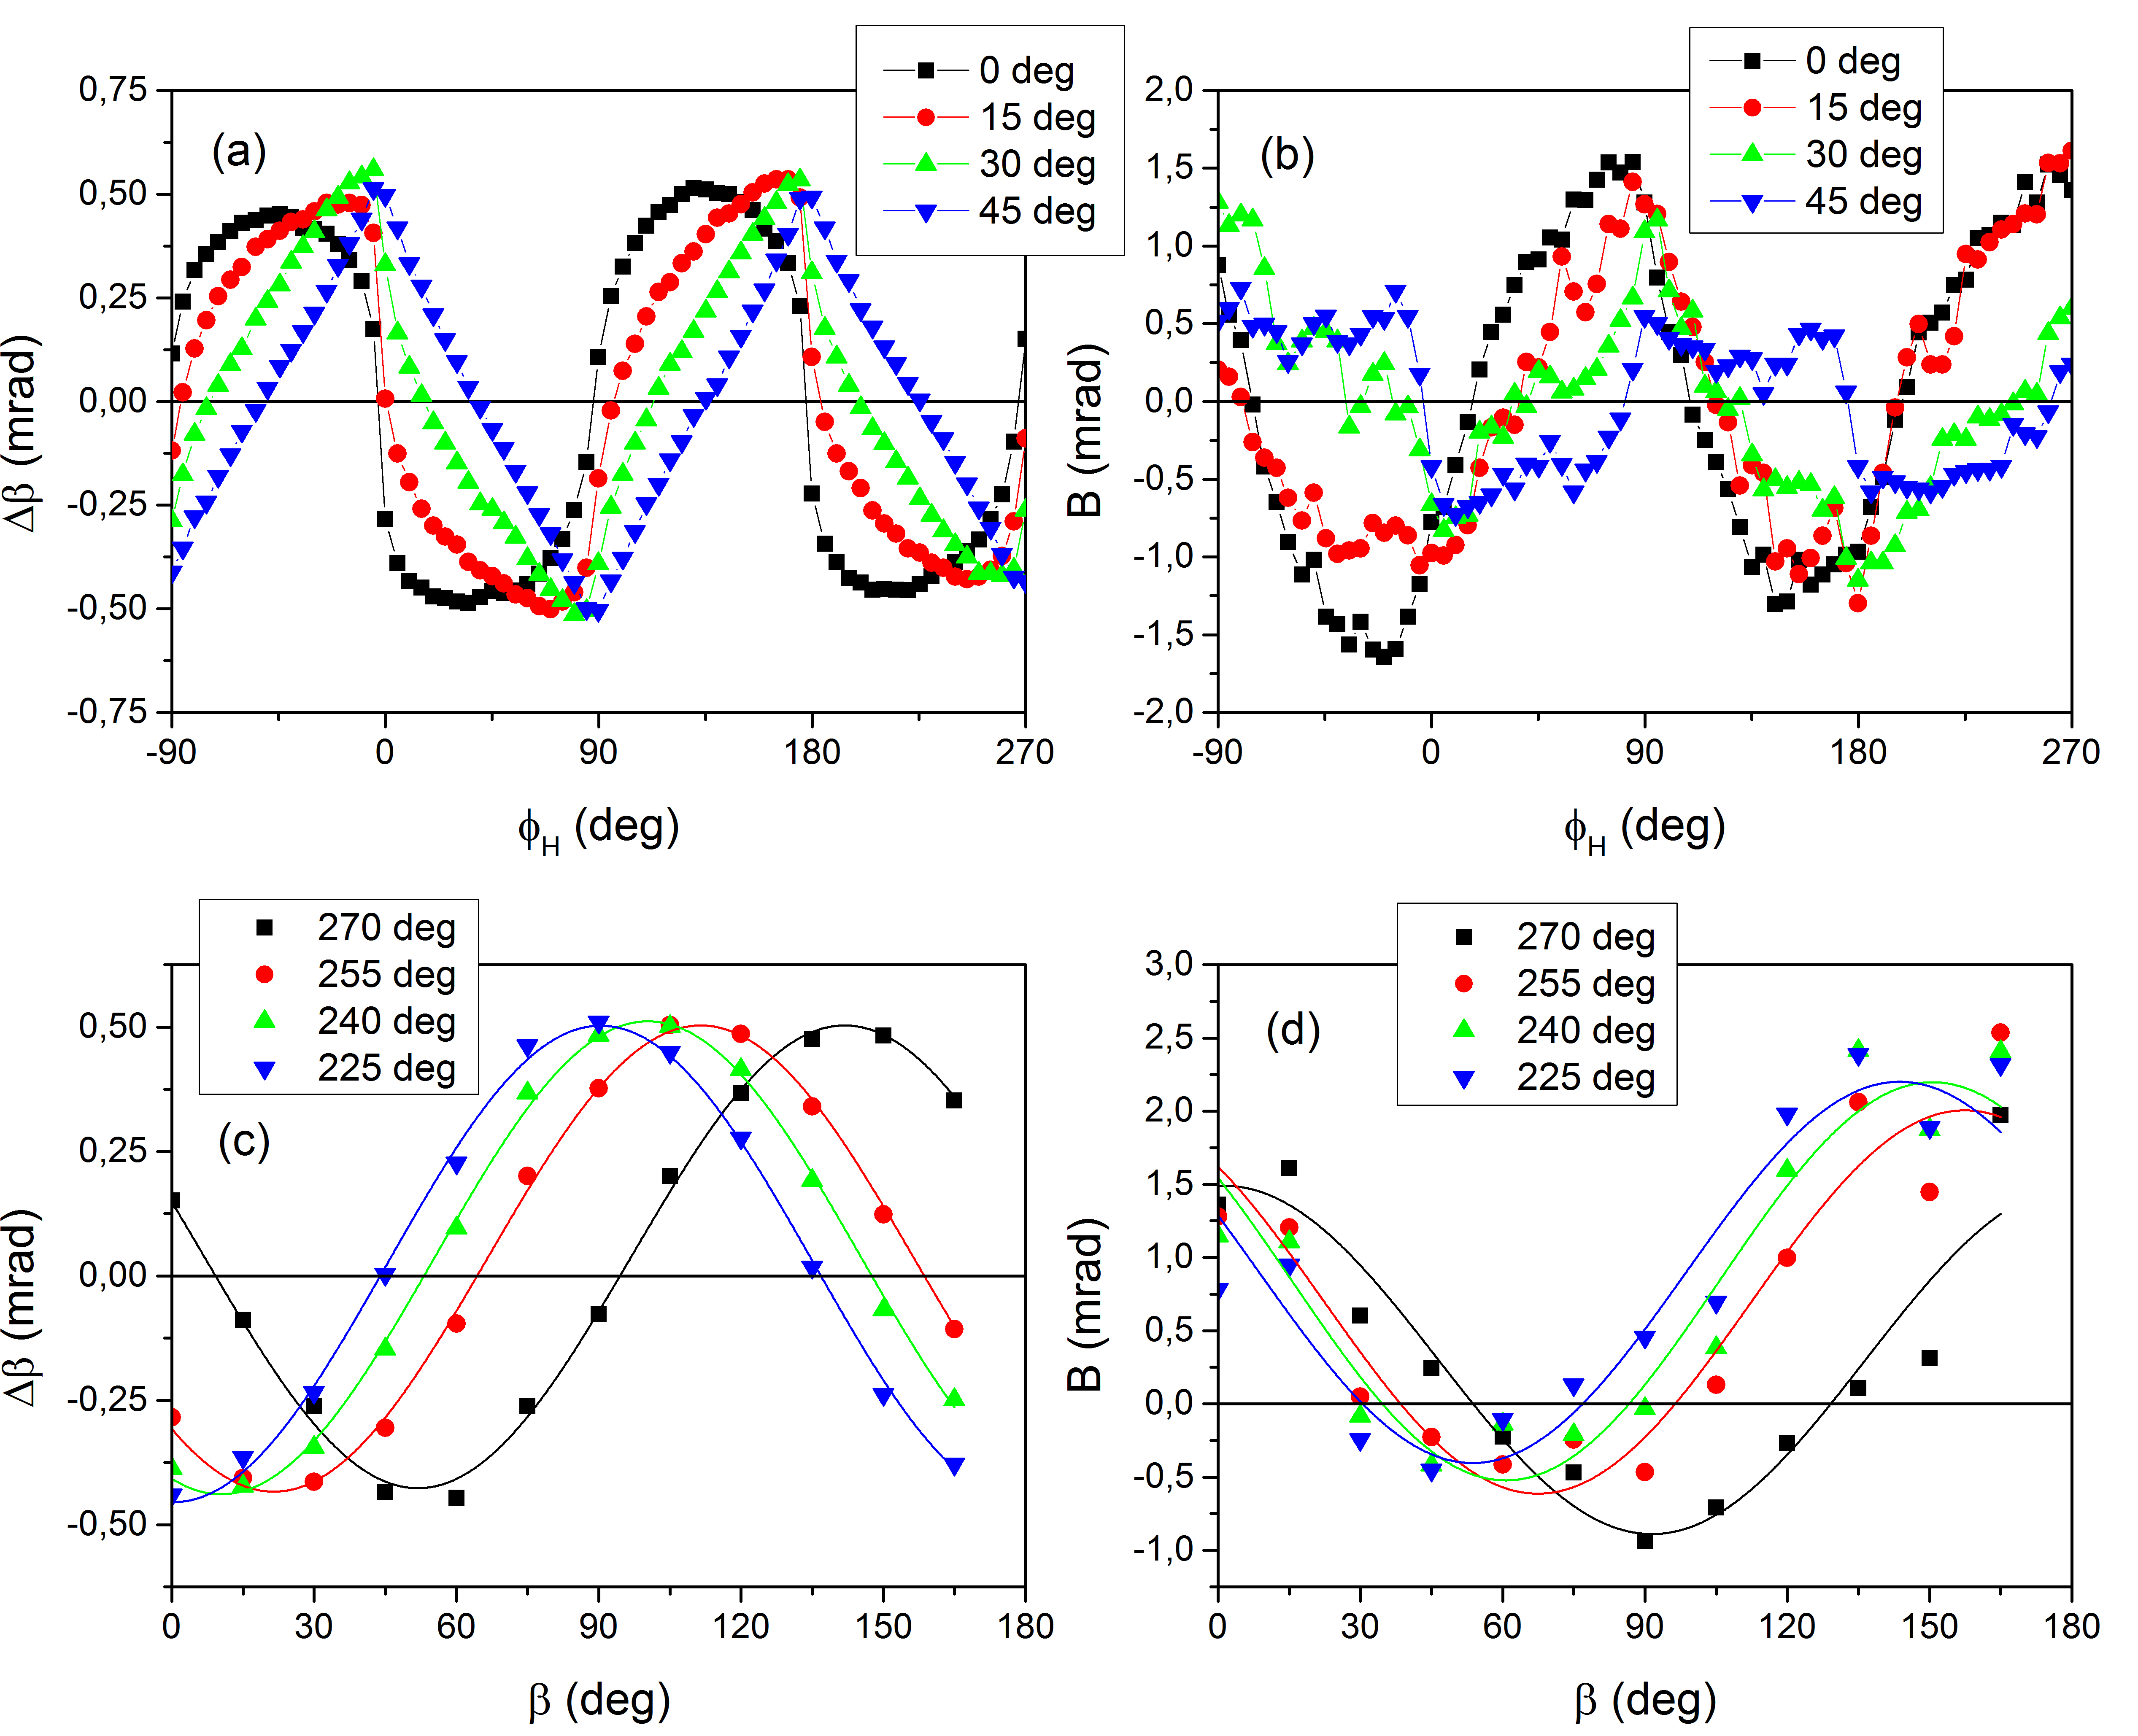
\includegraphics[width=\textwidth]{./png/graftoc_zpracovani}}
	\caption{Změna směru pole při jeho konstantní velikosti $\mu_0 \hext=\SI{210}{\milli\tesla}$ při $T<\SI{15}{\kelvin}$. (a) Voigtův jev pro vybrané polarizace. (b) MLD pro vybrané polarizace. (c) Přeskládaná data pro vybrané směry pole $\phH$ --- Voigtův jev, (d) MLD}\label{toc_hrube}
\end{figure}

Naměřená data mají nezávislou proměnnou $\phH$ a parametr $\beta$. Přeskládáme je tak, aby nezávislá proměnná byla $\beta$ a parametr $\phH$ jako na obr. \ref{toc_hrube} (c), (d).
Získané závislosti dále fitujeme funkcemi \eqref{e:asass} a \eqref{e:sss}. Poměrně často, především v $B$, však dochází k tomu, že závislost má zřetelně harmonický průběh, ale je posunutá (viz obr. \ref{toc_preskladane} (a)). Proto závislosti fitujeme také funkcemi s přidaným absolutním členem
\begin{equation} \label{e:tocsc}
\begin{aligned}
\Delta \beta(\phH, \beta) &= \pmld \sin \left[ 2(\phM(\phH)-\beta) \right]+c \,, \\
B(\phH, \beta) &= 2 \left(\pmld \cos \left[ 2(\phM(\phH)-\beta) \right]+c \right) \,.
\end{aligned}
\end{equation}
Výsledné $\phM$ a $\pmld$ z fitu s absolutním členem a bez jsou ve všech případech od sebe nerozeznatelné, pouze nejistota fitu je s absolutním členem mnohem menší.

\begin{figure}[htbp]\centering
\qq{	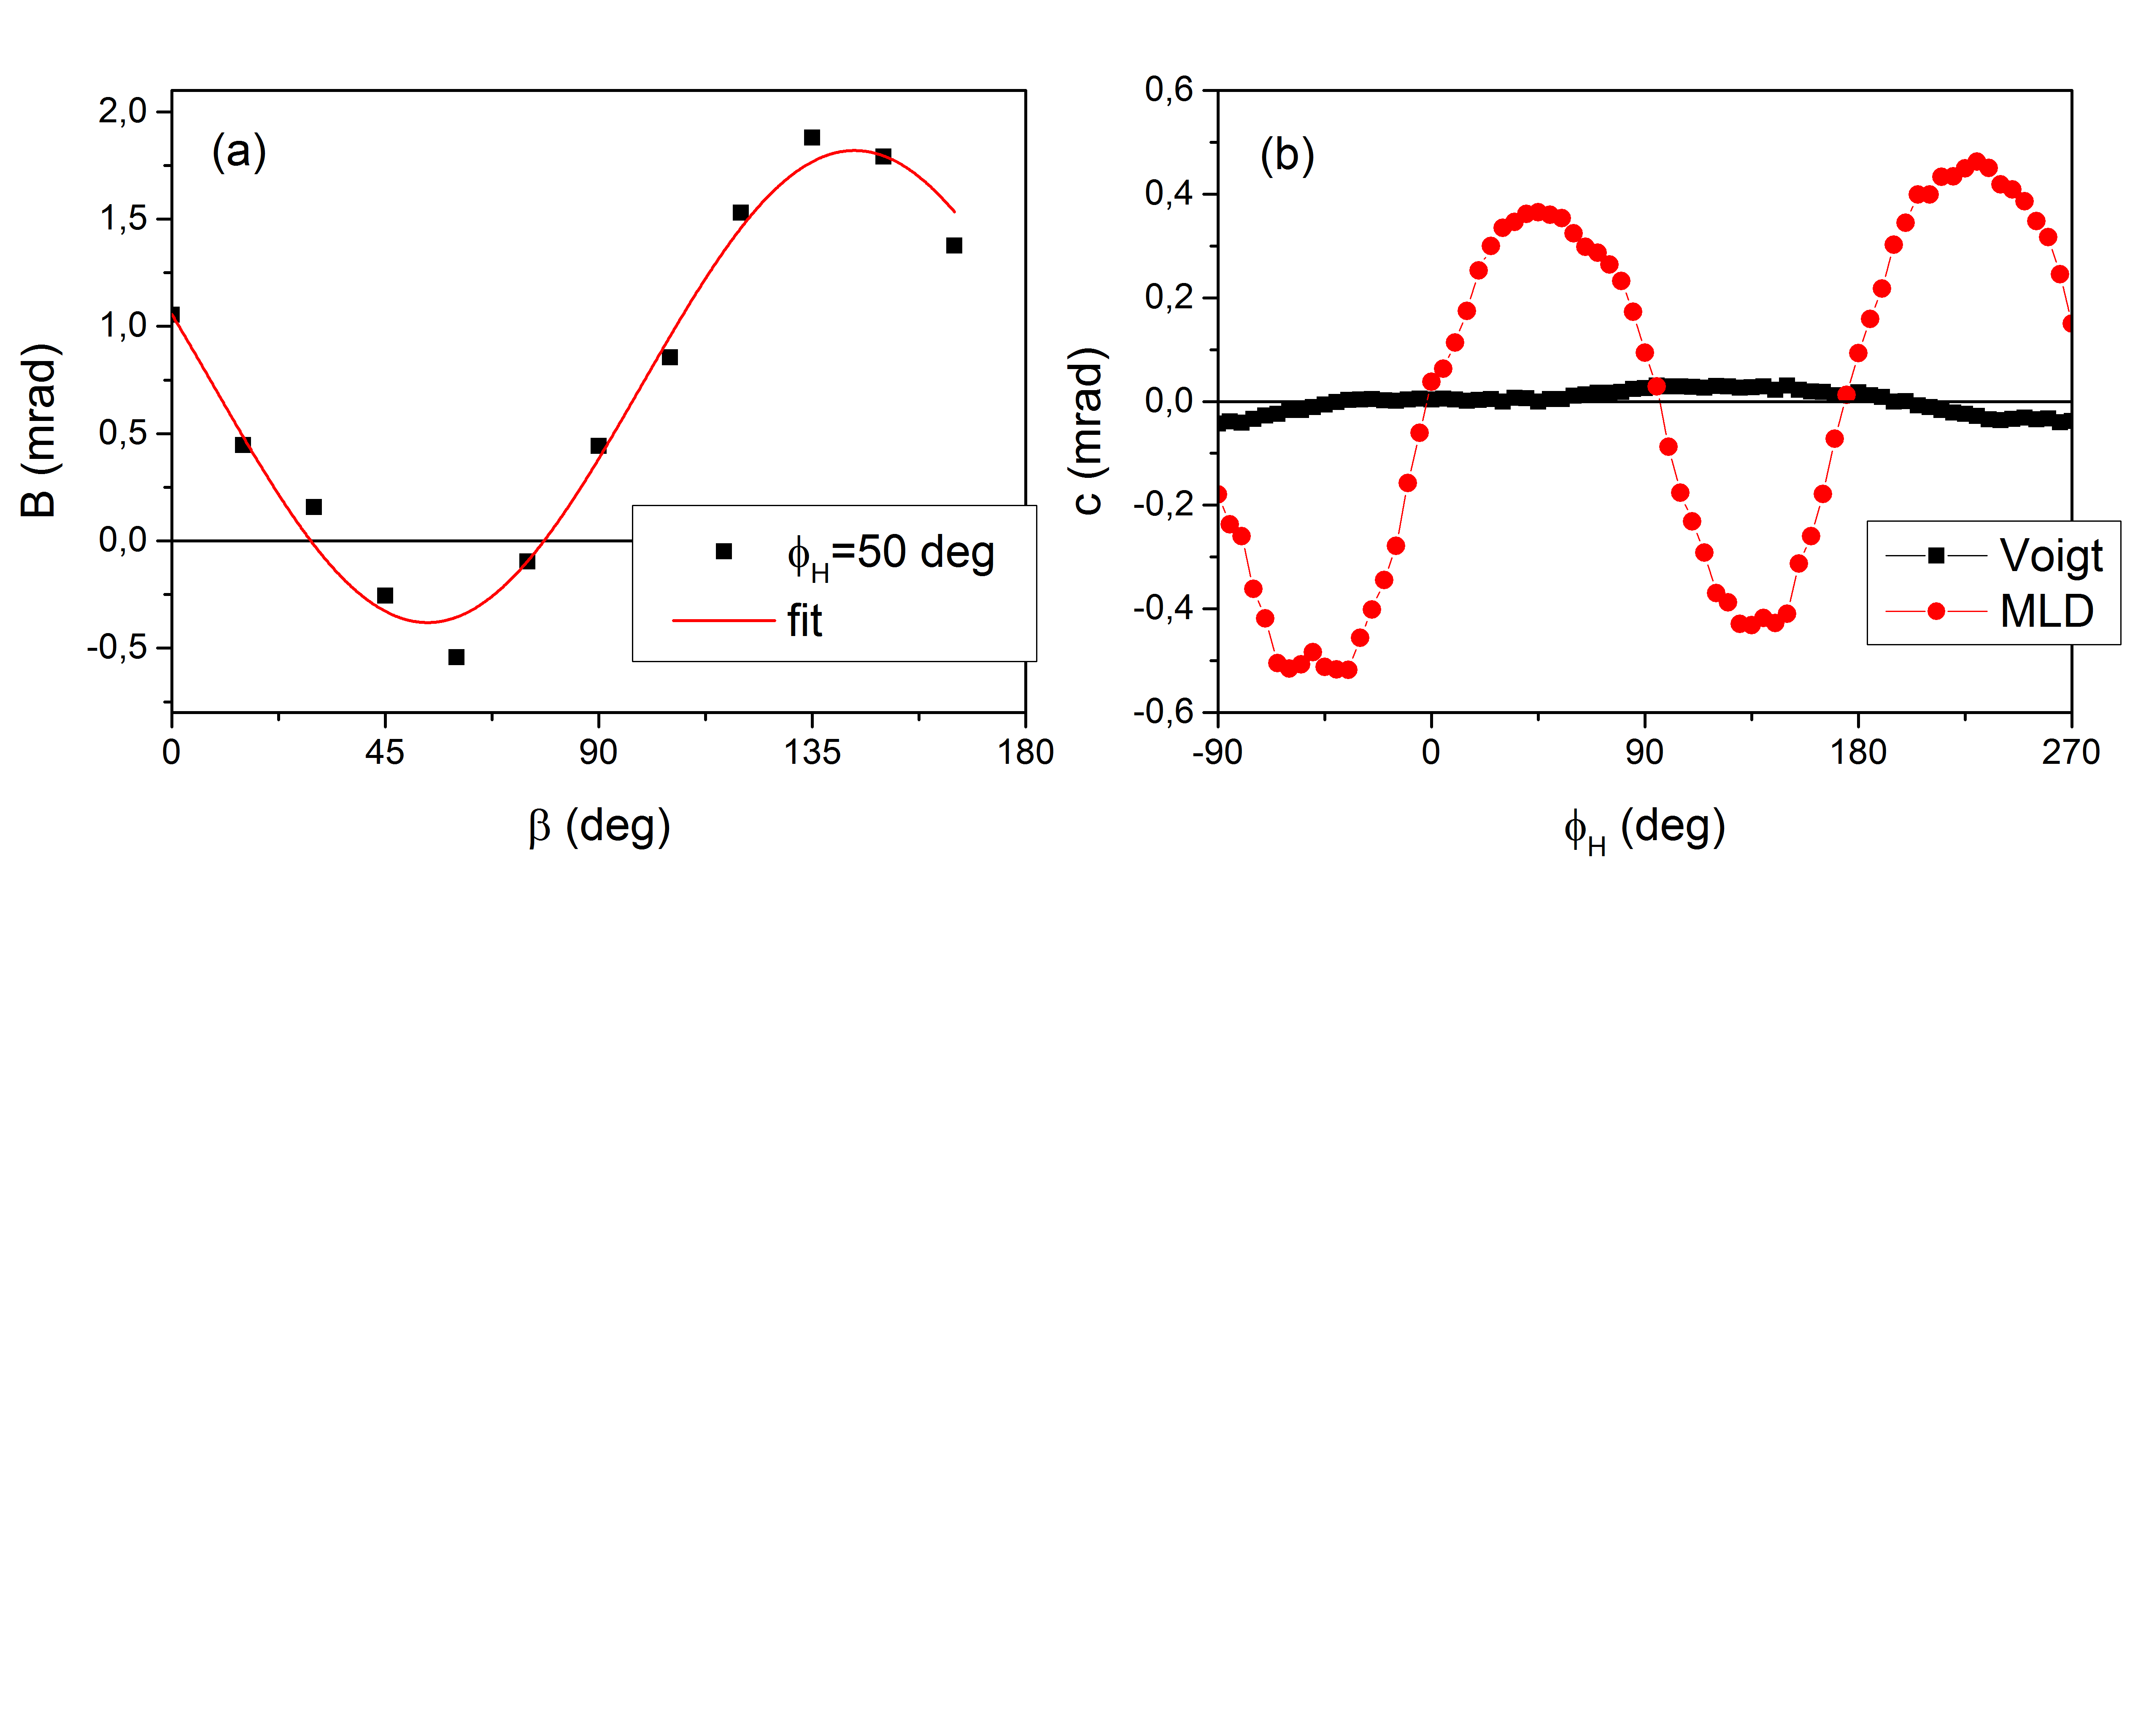
\includegraphics[trim={0 3.43in 0 0}, clip, width=\textwidth]{./png/graftoc_preskladane}}
	\caption{Změna směru pole při jeho konstantní velikosti $\mu_0 \hext=\SI{210}{\milli\tesla}$ při $T<\SI{15}{\kelvin}$. (a) Příklad přeskládaných dat s nenulovým absolutním členem. (b) Fitované absolutní členy $c$.}\label{toc_preskladane}
\end{figure}

\section{Výsledky}

Hlavními výsledky těchto experimentů jsou závislosti $\phM(\phH)$ a $\pmld(\phM)$.
Na obr. \ref{toc_vysledkyuhel} jsou grafy závislostí $\phM(\phH)$, pro každý směr pole je vynesena hodnota $\phM-\phH$, tj. úhel, který spolu svírá magnetizace a pole.

Pokud by pole bylo podstatně silnější než magnetická anizotropie ve vzorku, magnetizace by vždy mířila do směru pole a na grafu bychom pozorovali kružnici $\phM-\phH=\ang{0}$. Z grafu \ref{toc_vysledkyuhel} (a) je patrné, že při $T<\SI{15}{\kelvin}$ není tato podmínka splněna ani pro $\mu_0\hext=\SI{210}{\milli\tesla}$. Při $\hext=\SI{50}{\milli\tesla}$ (obr. \ref{toc_vysledkyuhel} (b)) je efekt ještě výraznější, v nespojitostech dochází k přeskoku mezi snadnými osami. Z~těchto změřených závislostí je možné jednoznačně určit polohu snadných os magnetizace ve vzorku (body $\phM=\phH$). Z obr. \ref{toc_vysledkyuhel} (b) můžeme tedy určit, že ve studovaném vzorku F002 se tyto osy nacházejí ve směrech $\num{45(5)}^\circ$ a $\num{136(5)}^\circ$, což vzhledem ke krystalografickému směru [100] (stejně jako v tabulce \ref{tab_vzorek}) odpovídá úhlům $\num{90(7)}^\circ$ a $\num{181(7)}^\circ$. Dříve provedená měření magnetické anizotropie v tomto vzorku, která byla uskutečněna pomocí laserovými pulzy vyvolané precese magnetizace \cite{TesarovaDisertace} vedla k závěru, že tyto snadné směry se nacházejí pro úhly $\num{104(5)}^\circ$ a $\num{166(5)}^\circ$ (viz tabulka \ref{tab_vzorek}). Tyto hodnoty se sice ani v rámci chyby měření neshodují, ale nejsou příliš odlišné. Je velice pravděpodobné, že jejich polohu umožňuje přesněji určit metoda popsaná v této práci.
Při vyšší teplotě (obr. \ref{toc_vysledkyuhel} (c)) se křivka mnohem více podobá kružnici. Dochází k měknutí anizotropie a magnetizace přesněji kopíruje směr pole.

Z grafů je též zřejmé, že měření pomocí Voigtova jevu je výrazně přesnější než MLD, což není překvapivé vzhledem k vyšší zašuměnosti součtového signálu (porovnejte \ref{toc_hrube} (a) a (b)).
Dále proto pro úhlovou závislost $\pmld(\phM)$ používáme pouze nafitované $\phM(\phH)$ z Voigtova jevu.
Hlavní výhoda měření i součtového signálu (MLD) je to, že nám umožňuje snadno určit znaménko $\pmld$.

Na obr. \ref{toc_vysledkypmld} (a) je úhlová závislost $\pmld(\phM)$ při $T<\SI{15}{\kelvin}$ při velikostech pole $\mu_0\hext=\SI{210}{\milli\tesla}$ a \SI{50}{\milli\tesla}. Obě velikosti pole dávají podle očekávání stejné $\pmld$. Při nižším poli procházel směr magnetizace menším rozsahem úhlů, a tak máme hodnoty jen pro směry v těsné blízkosti snadných os. V grafu je pro ilustraci též vyneseno nafitované $\pmld$ z MLD při $\mu_0\hext=\SI{210}{\milli\tesla}$. I v případě urční $\pmld$ vede měření Voigtova jevu k podstatně menší chybě než měření MLD.

Na obr. \ref{toc_vysledkypmld} (b) je opět graf úhlové závislosti $\pmld$, tentokrát pro $\mu_0\hext=\SI{210}{\milli\tesla}$ a dvě různé teploty: \SI{12(3)}{\kelvin} a \SI{38,7(10)}{\kelvin}. Při vyšší teplotě dochází vlivem nižší magnetizace ke snížení $|\pmld|$. V obou případech je zde ale jasně patrná směrová závislost $\pmld$: Největší hodnotu $\pmld$ dosahuje pro $\phM\approx \ang{0}$ (resp. \ang{180}), což odpovídá krystalografickému směru [110]. Nejmenší hodnoty jsou naopak pro $\phM\approx \ang{45}+n\cdot \ang{90}$, kde $n$ je celé číslo, což odpovídá krystalografickým směrům [100] a [010]. Tato měření tedy umožňují od sebe oddělit na krystalografickém směru závislé a nezávislé složky magnetooptického koeficientu $\pmld$.

\begin{figure}[htbp]\centering
\qq{	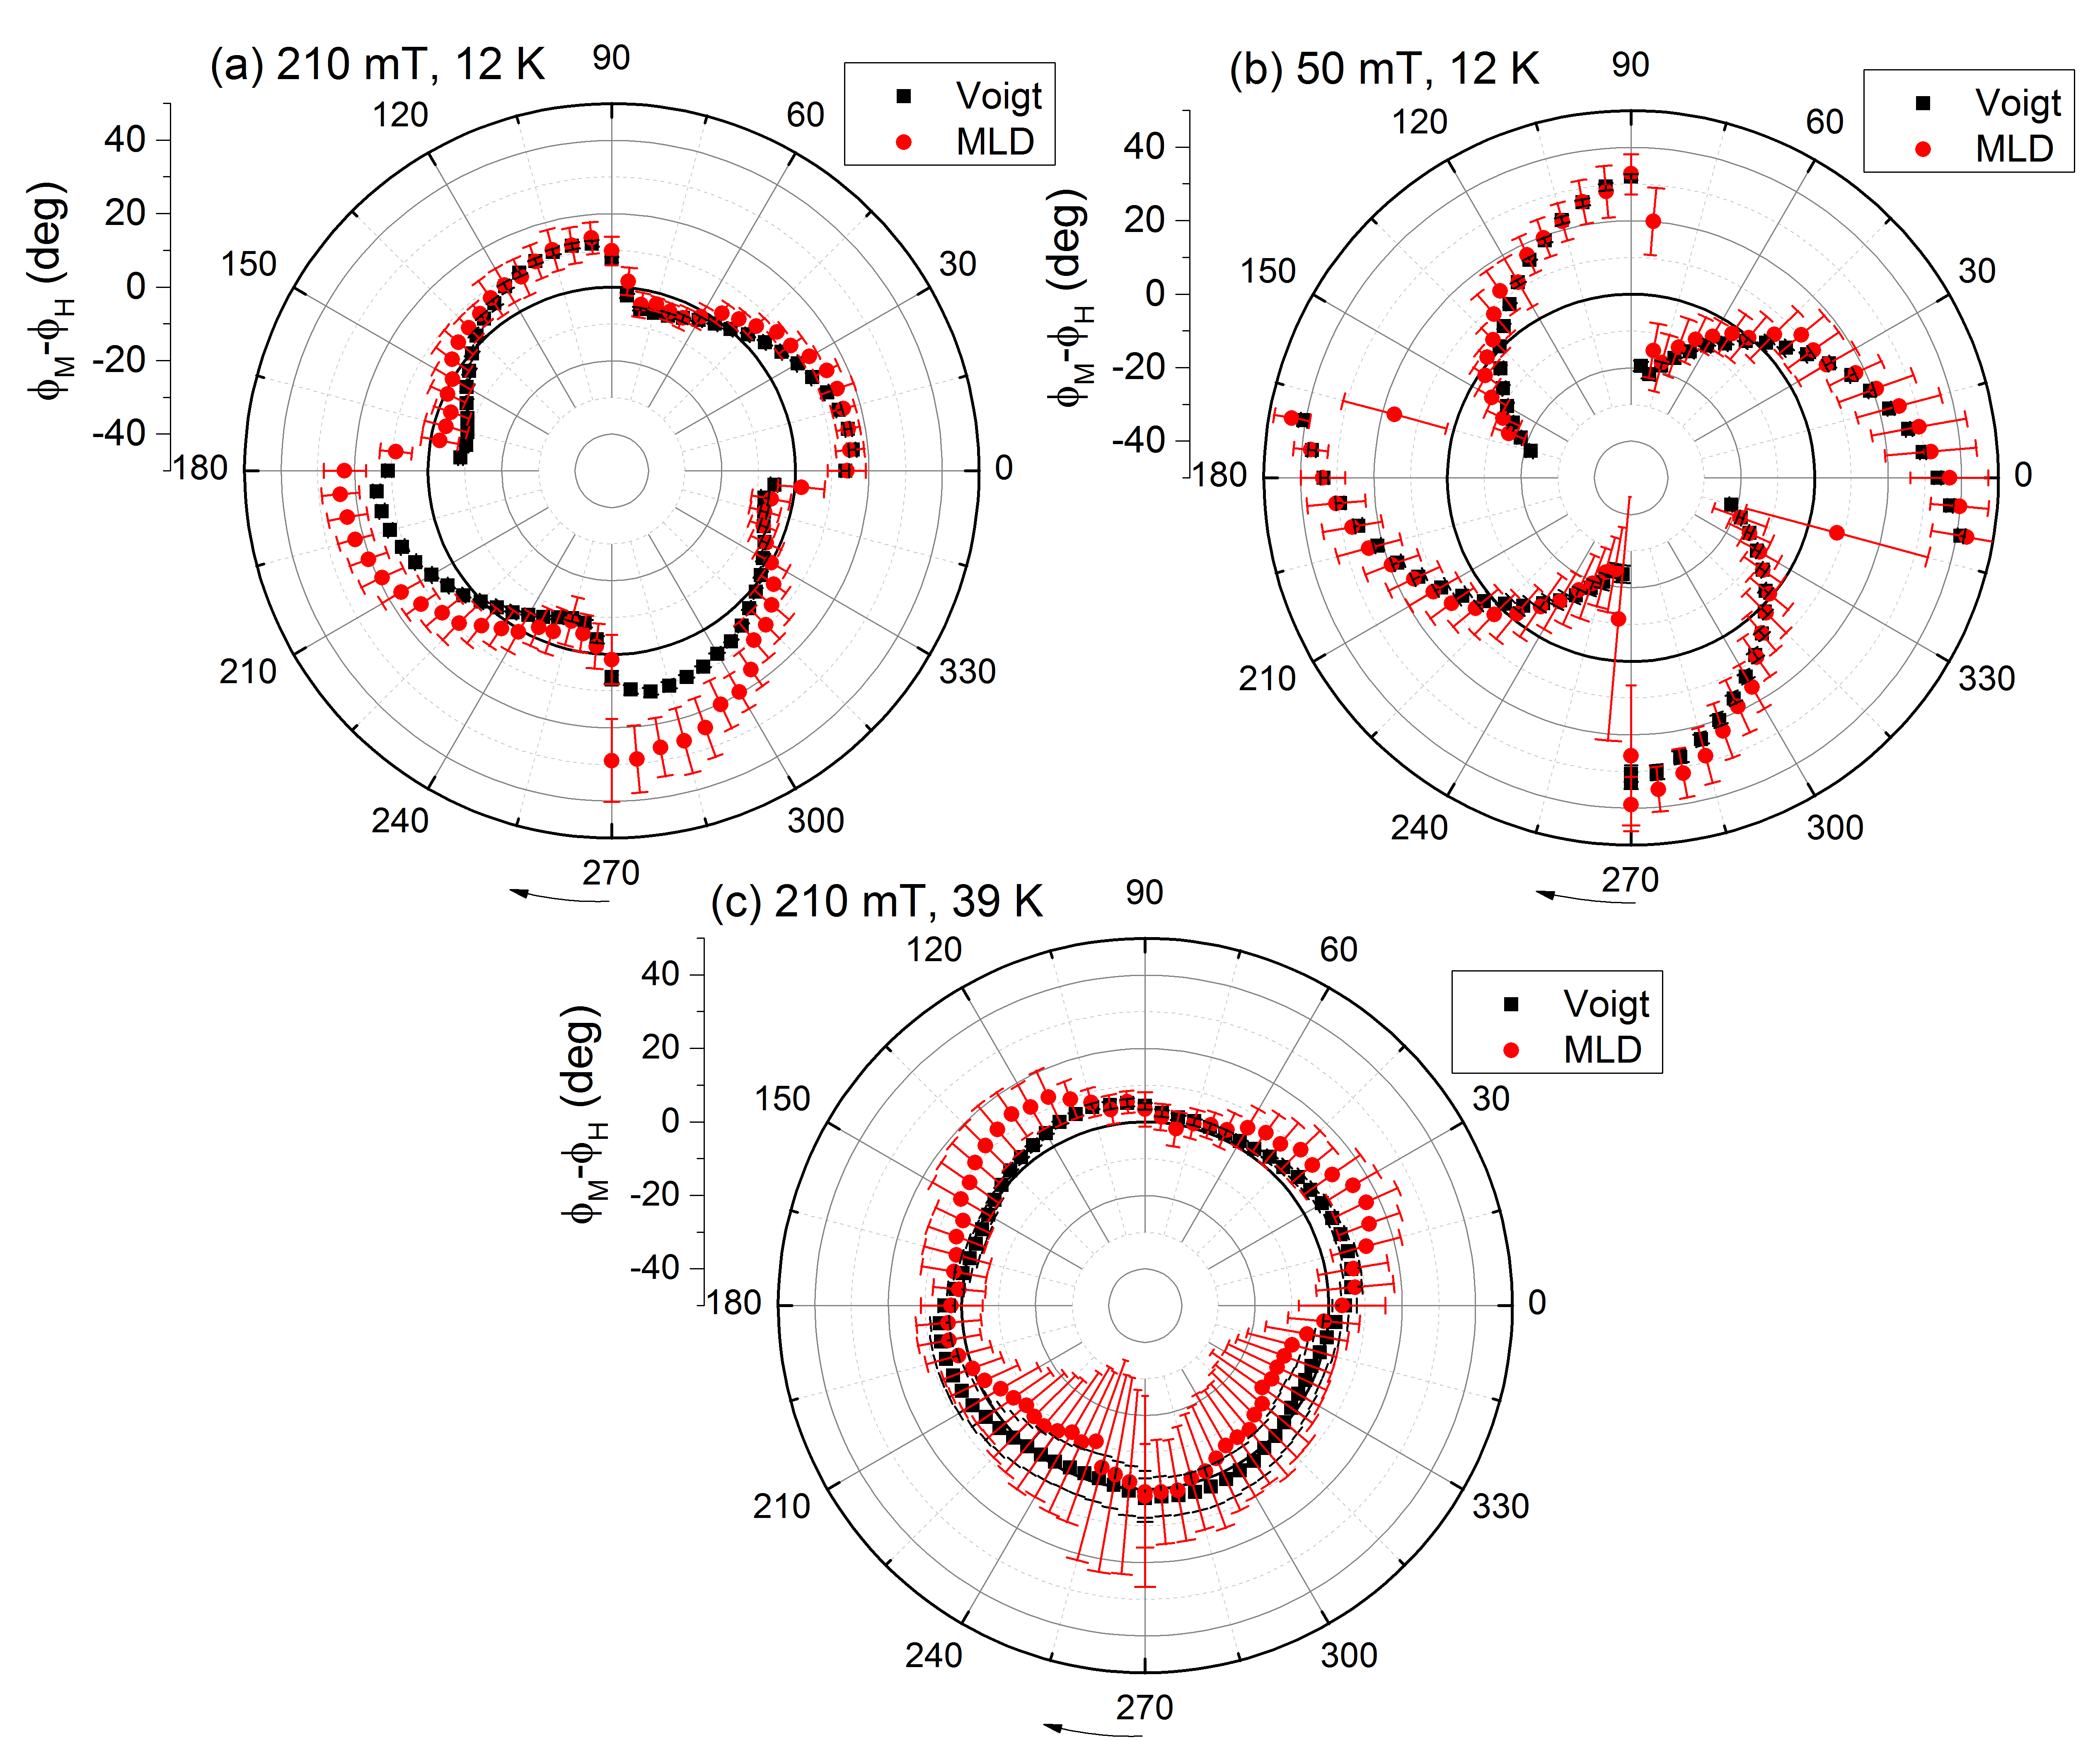
\includegraphics[width=\textwidth]{./png/tocgraf_uhly}}
	\caption{Změna směru pole při jeho konstantní velikosti. Závislost $\phM$ na směru vnějšího pole $\phH$. (a) $\hext=\SI{210}{\milli\tesla}$, $T<\SI{15}{\kelvin}$. (b) $\hext=\SI{50}{\milli\tesla}$, $T<\SI{15}{\kelvin}$. (c)  $\hext=\SI{210}{\milli\tesla}$, $T=\SI{38,7(10)}{\kelvin}$. }\label{toc_vysledkyuhel}
\end{figure}

\begin{figure}[htbp]\centering
\qq{	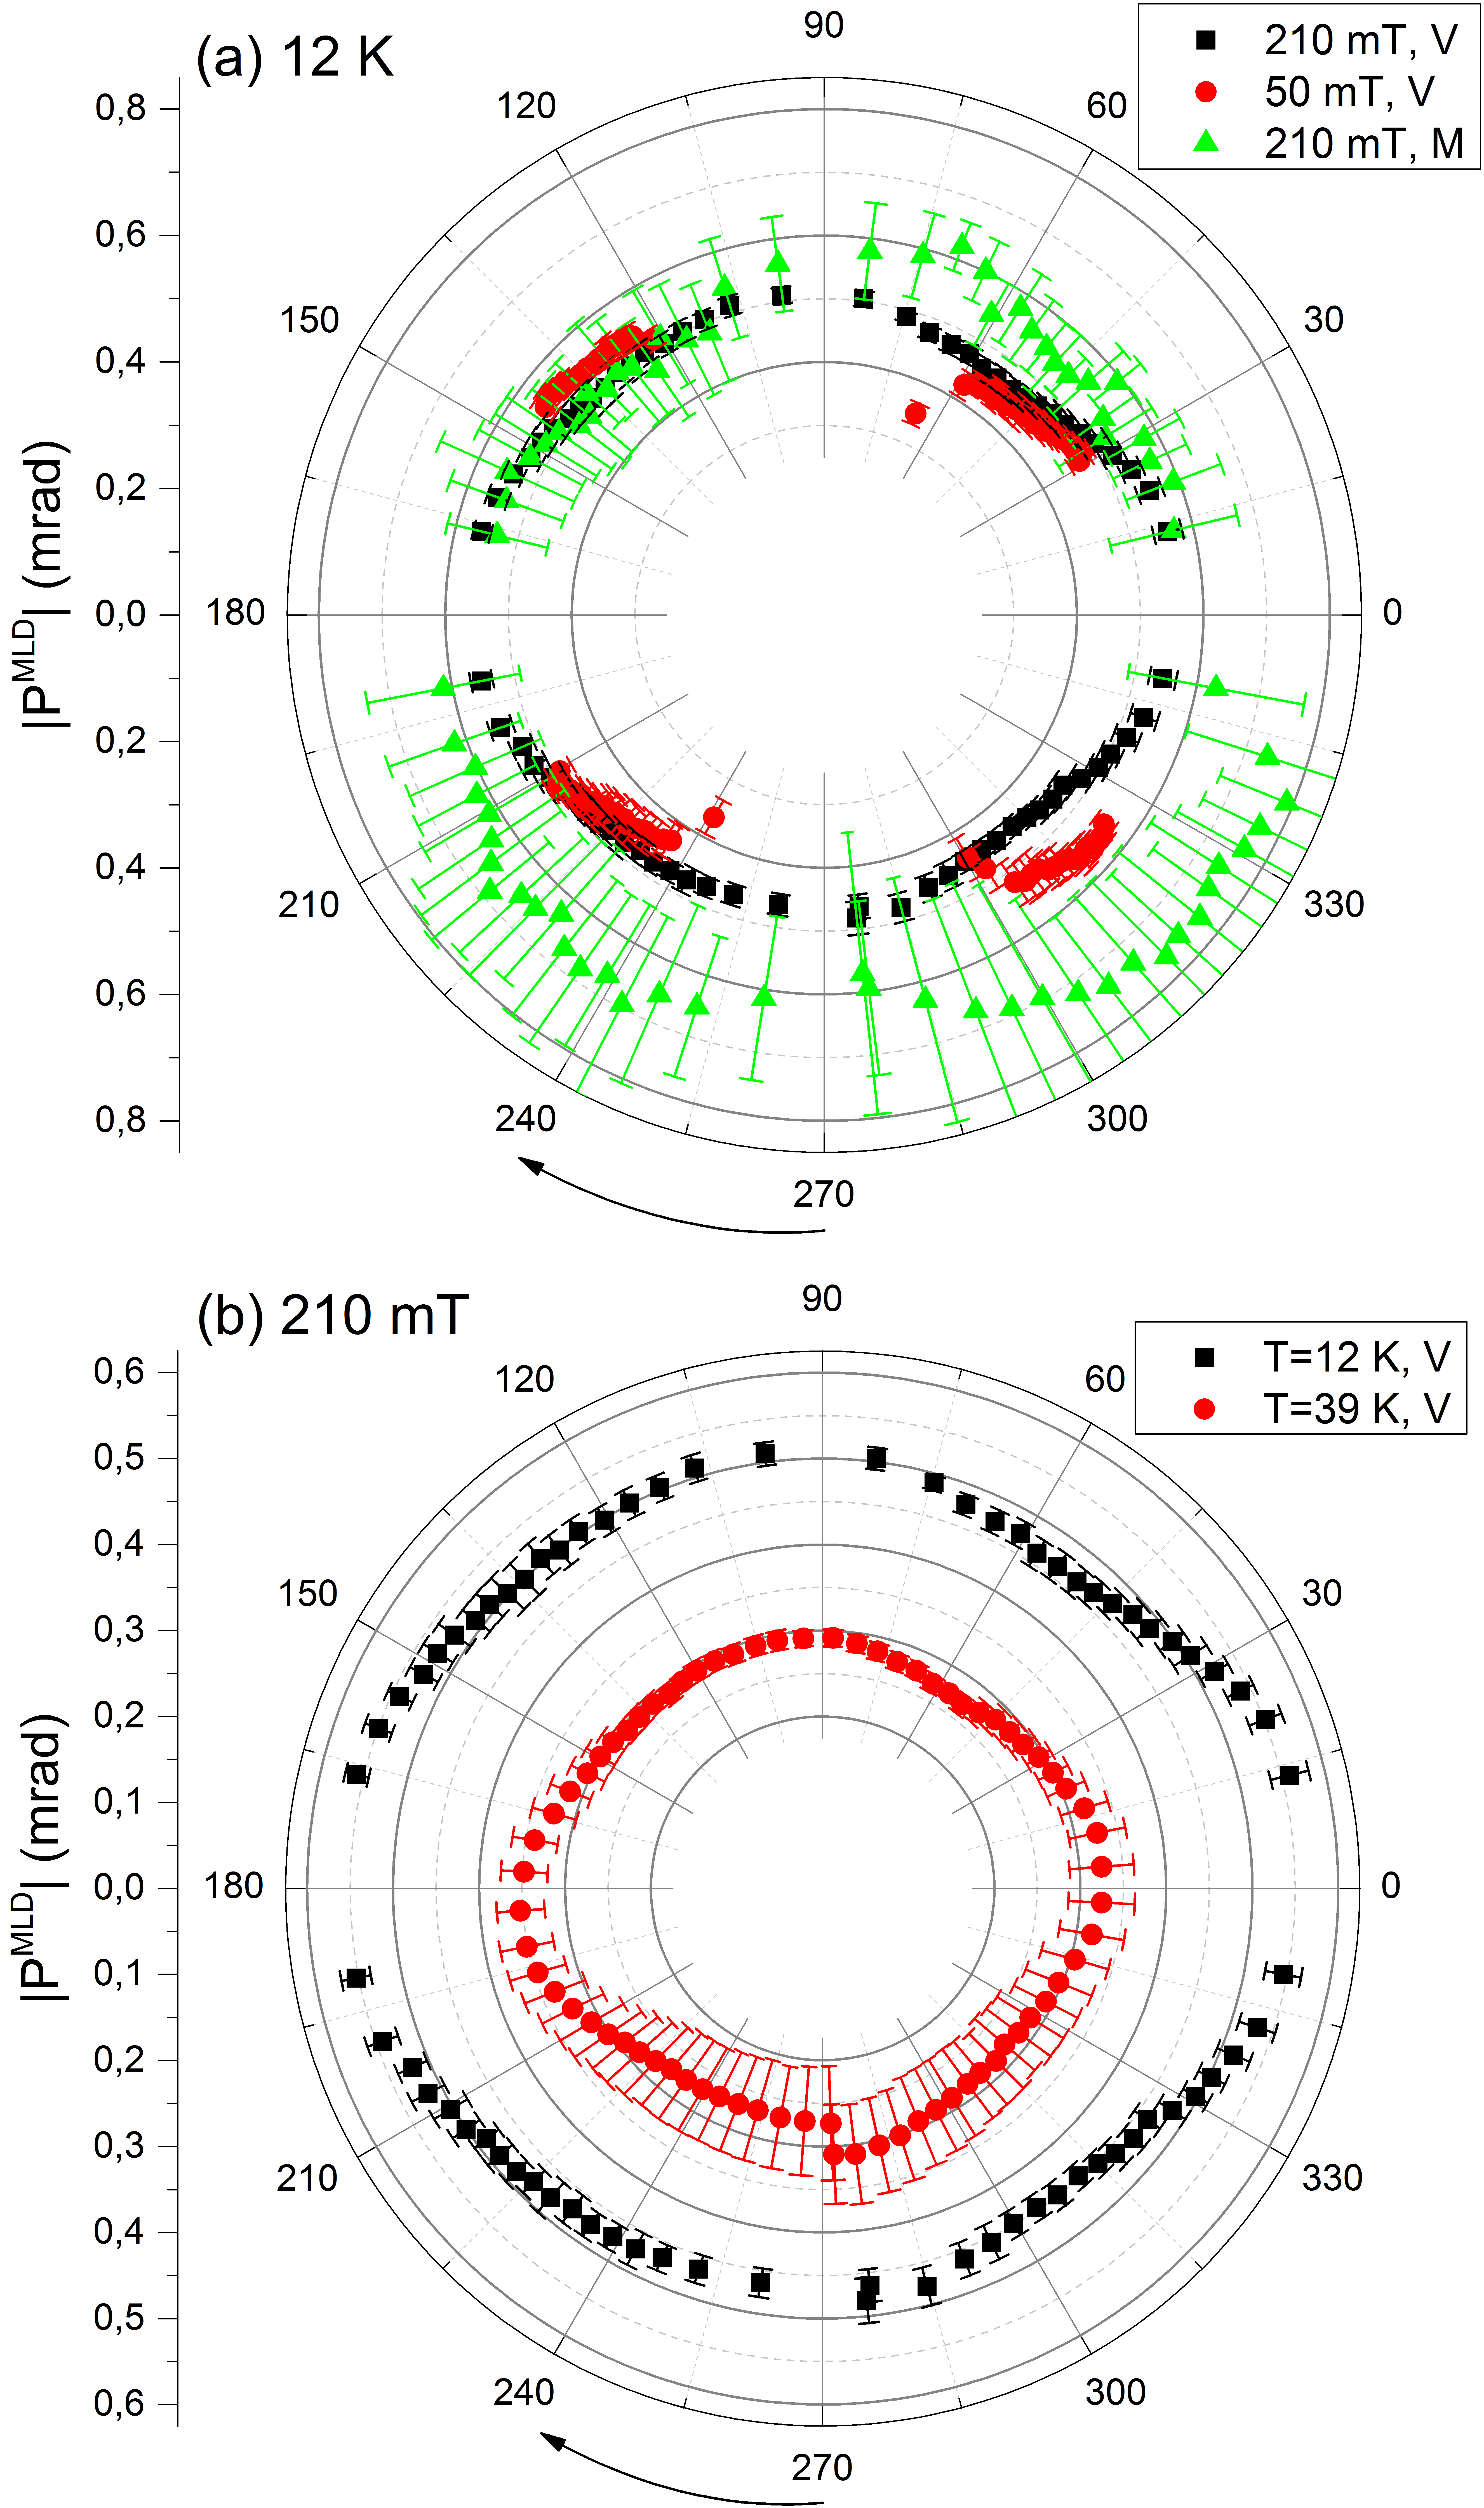
\includegraphics[width=0.8\textwidth]{./png/tocgraf_pmldvse}}
	\caption{Změna směru pole při jeho konstantní velikosti. Závislost nafitované $\pmld$ na směru magnetizace $\phM$ (viz. obr \ref{toc_vysledkyuhel}). $\pmld$ je záporné, v~grafu je vynesena absolutní hodnota. (a) Dvě různé velikosti pole $\hext$ při $T<\SI{15}{\kelvin}$. (b) $\mu_0\hext=\SI{210}{\milli\tesla}$ při dvou různých teplotách $T=\SI{12(3)}{\kelvin}$ a \SI{38,7(10)}{\kelvin}. V -- Voigtův jev, M -- MLD.}\label{toc_vysledkypmld}
\end{figure}